\documentclass{standalone}
\usepackage{tikz}
\usetikzlibrary{shapes,arrows,positioning,calc,decorations.pathreplacing}

% Define colors
\definecolor{inputblue}{RGB}{173,216,230}
\definecolor{encodergreen}{RGB}{144,238,144}
\definecolor{gnnred}{RGB}{255,182,193}
\definecolor{poolorange}{RGB}{255,165,0}
\definecolor{mlppurple}{RGB}{186,85,211}
\definecolor{outputblack}{RGB}{50,50,50}

\begin{document}
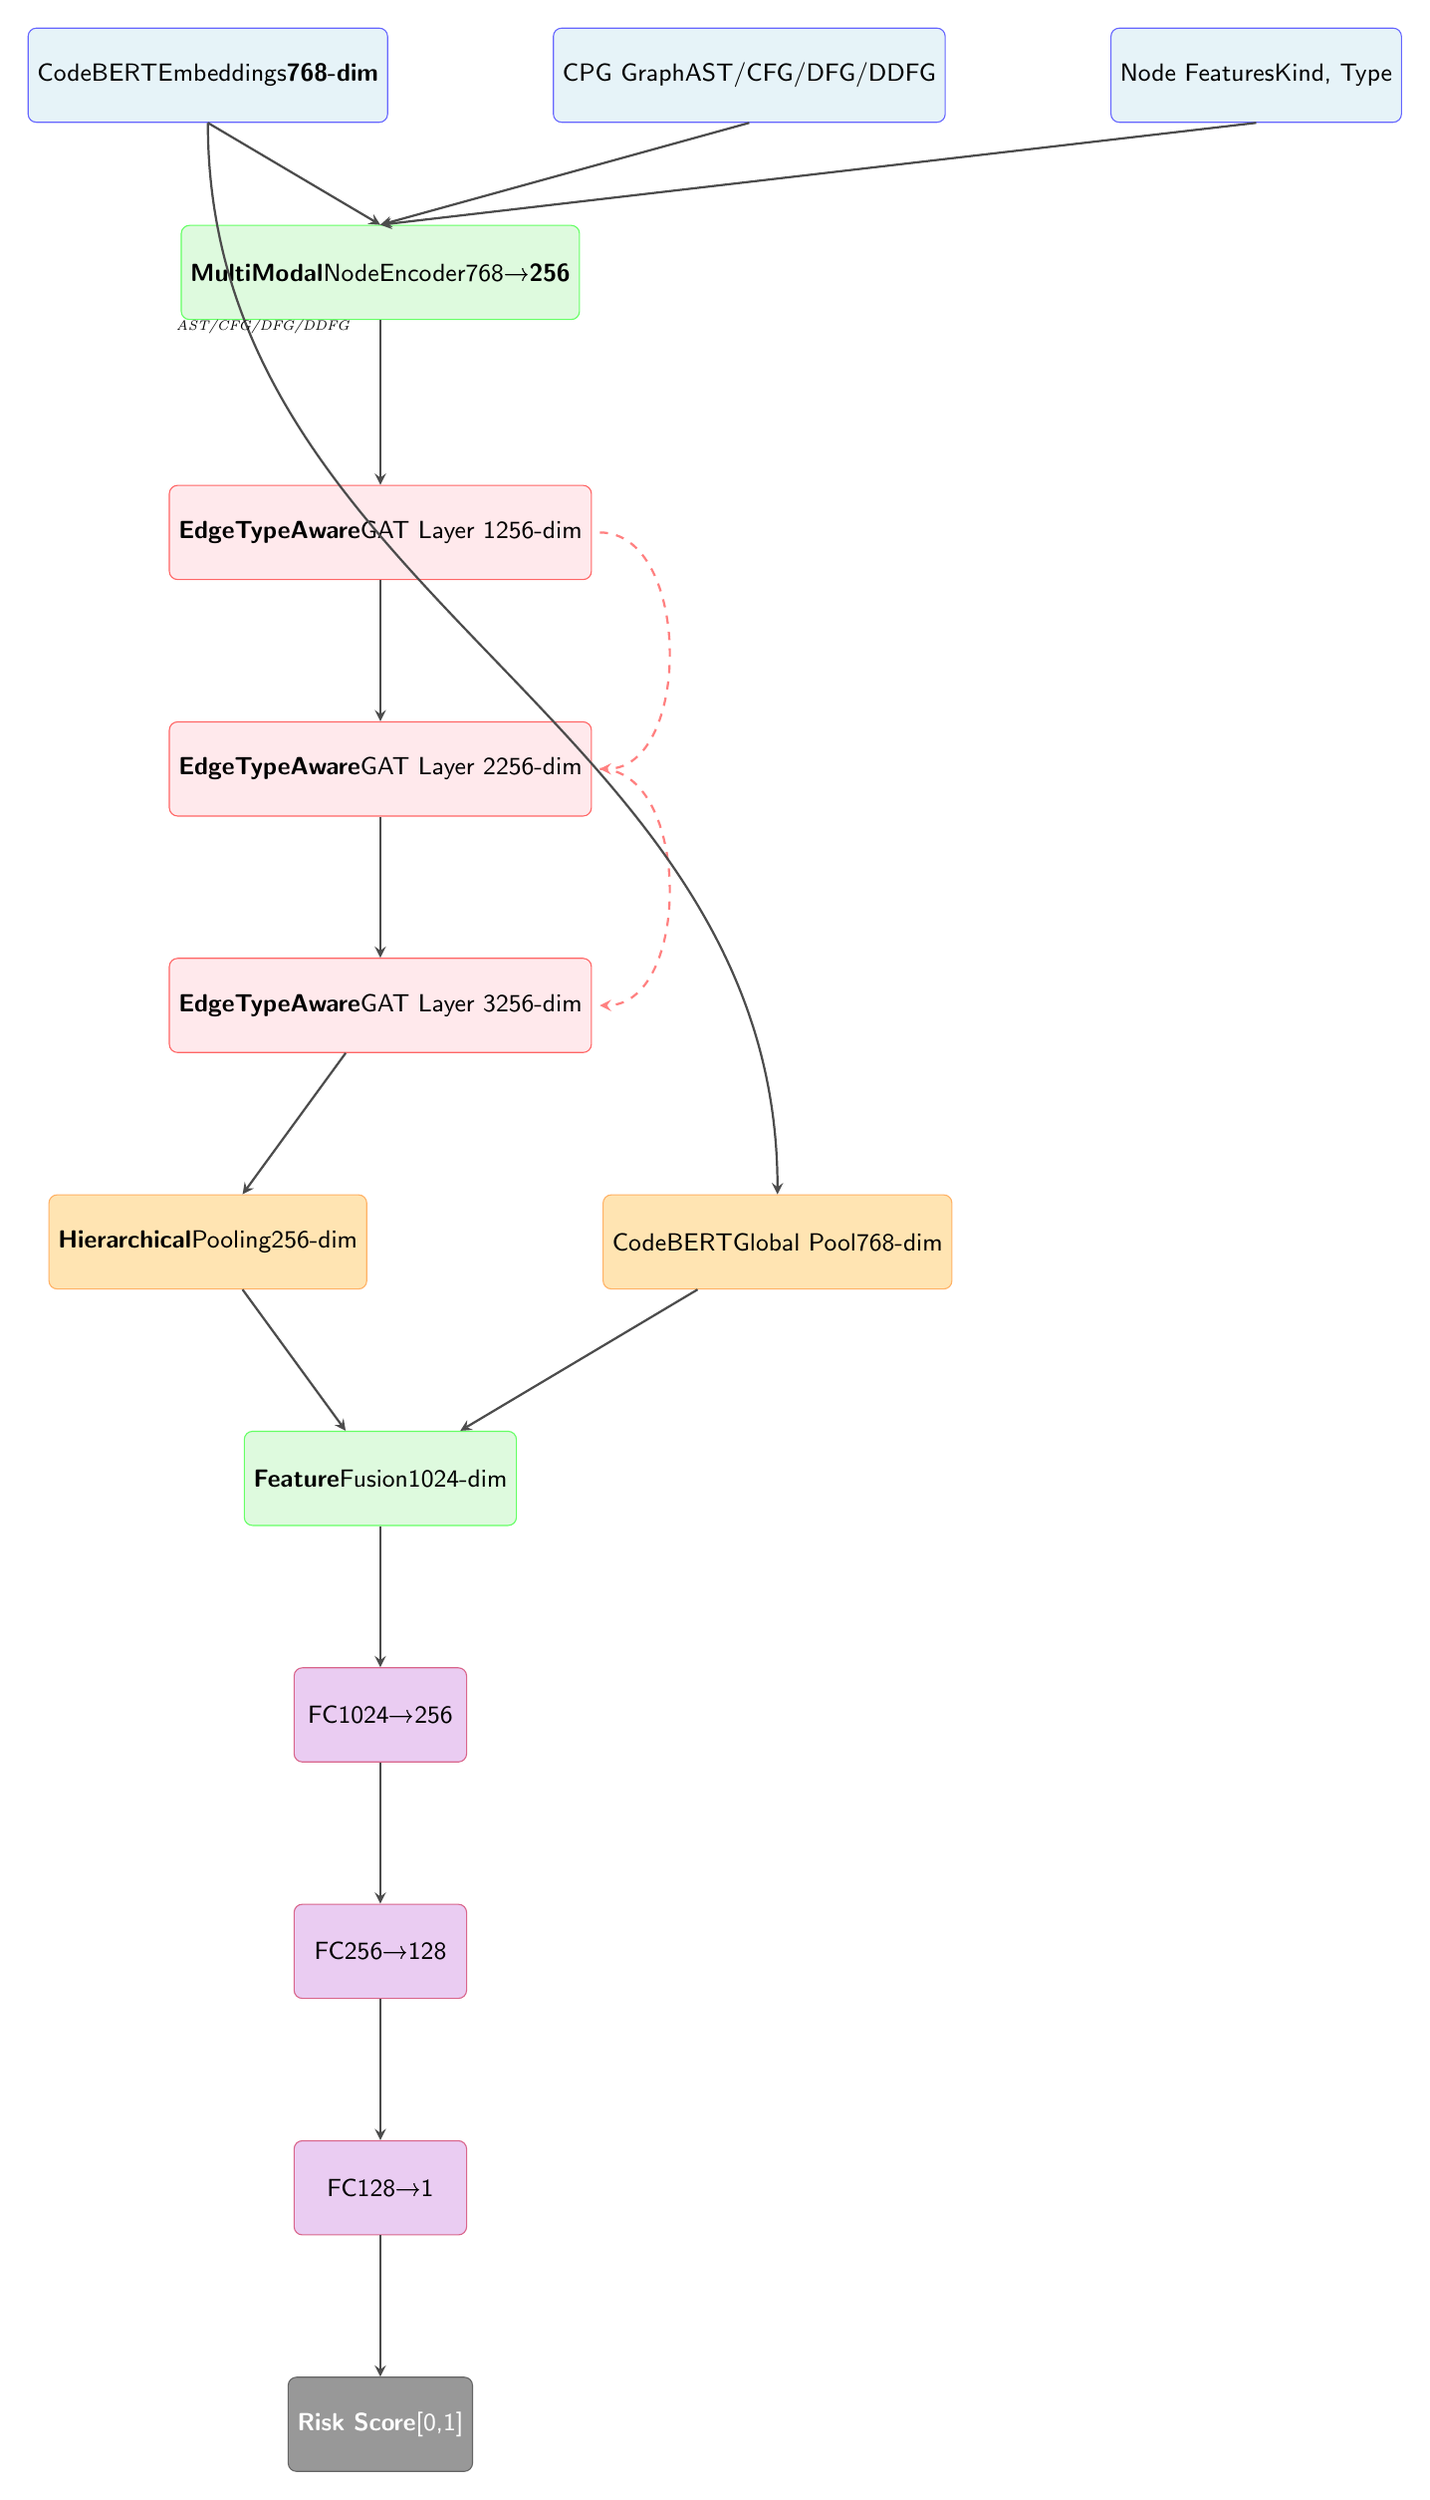
\begin{tikzpicture}[
    node distance=1.8cm,
    every node/.style={font=\small\sffamily},
    input/.style={rectangle, draw=blue!60, fill=inputblue!30, minimum width=2.2cm, minimum height=1.2cm, text centered, rounded corners=3pt},
    encoder/.style={rectangle, draw=green!60, fill=encodergreen!30, minimum width=2.2cm, minimum height=1.2cm, text centered, rounded corners=3pt},
    gnn/.style={rectangle, draw=red!60, fill=gnnred!30, minimum width=2.2cm, minimum height=1.2cm, text centered, rounded corners=3pt},
    pool/.style={rectangle, draw=orange!60, fill=poolorange!30, minimum width=2.2cm, minimum height=1.2cm, text centered, rounded corners=3pt},
    mlp/.style={rectangle, draw=purple!60, fill=mlppurple!30, minimum width=2.2cm, minimum height=1.2cm, text centered, rounded corners=3pt},
    output/.style={rectangle, draw=black!60, fill=outputblack!50, minimum width=2.2cm, minimum height=1.2cm, text centered, rounded corners=3pt, text=white},
    arrow/.style={->, >=stealth, thick, color=black!70},
    residual/.style={->, >=stealth, thick, color=red!50, dashed}
]

% Input layer
\node[input] (codebert) {CodeBERT\\Embeddings\\\textbf{768-dim}};
\node[input, right=of codebert, xshift=0.3cm] (cpg) {CPG Graph\\AST/CFG/DFG/DDFG};
\node[input, right=of cpg, xshift=0.3cm] (nodefeat) {Node Features\\Kind, Type};

% Encoder
\node[encoder, below=of codebert, xshift=2.2cm, yshift=0.5cm] (encoder) {\textbf{MultiModal}\\NodeEncoder\\768→\textbf{256}};

% GNN layers
\node[gnn, below=of encoder, yshift=-0.3cm] (gnn1) {\textbf{EdgeTypeAware}\\GAT Layer 1\\256-dim};
\node[gnn, below=of gnn1] (gnn2) {\textbf{EdgeTypeAware}\\GAT Layer 2\\256-dim};
\node[gnn, below=of gnn2] (gnn3) {\textbf{EdgeTypeAware}\\GAT Layer 3\\256-dim};

% Pooling
\node[pool, below=of gnn3, xshift=-2.2cm] (hierpool) {\textbf{Hierarchical}\\Pooling\\256-dim};
\node[pool, right=of hierpool, xshift=1.2cm] (codebertpool) {CodeBERT\\Global Pool\\768-dim};

% Fusion
\node[encoder, below=of hierpool, xshift=2.2cm] (fusion) {\textbf{Feature}\\Fusion\\1024-dim};

% MLP layers
\node[mlp, below=of fusion] (mlp1) {FC\\1024→256};
\node[mlp, below=of mlp1] (mlp2) {FC\\256→128};
\node[mlp, below=of mlp2] (mlp3) {FC\\128→1};

% Output
\node[output, below=of mlp3] (output) {\textbf{Risk Score}\\{[0,1]}};

% Connections from input to encoder
\draw[arrow] (codebert.south) -- (encoder.north);
\draw[arrow] (cpg.south) -- (encoder.north);
\draw[arrow] (nodefeat.south) -- (encoder.north);

% Connections through GNN layers
\draw[arrow] (encoder) -- (gnn1);
\draw[arrow] (gnn1) -- (gnn2);
\draw[arrow] (gnn2) -- (gnn3);

% Residual connections
\draw[residual] ($(gnn1.east)+(0.1,0)$) to[out=0,in=0] ($(gnn2.east)+(0.1,0)$);
\draw[residual] ($(gnn2.east)+(0.1,0)$) to[out=0,in=0] ($(gnn3.east)+(0.1,0)$);

% Connections to pooling
\draw[arrow] (gnn3) -- (hierpool);
\draw[arrow] (codebert.south) to[out=-90,in=90] (codebertpool.north);

% Connections to fusion
\draw[arrow] (hierpool) -- (fusion);
\draw[arrow] (codebertpool) -- (fusion);

% Connections through MLP
\draw[arrow] (fusion) -- (mlp1);
\draw[arrow] (mlp1) -- (mlp2);
\draw[arrow] (mlp2) -- (mlp3);
\draw[arrow] (mlp3) -- (output);

% Add labels for edge types
\node[above=of gnn1, xshift=-1.5cm, font=\tiny\itshape] {AST/CFG/DFG/DDFG};

\end{tikzpicture}
\end{document}
